\documentclass[a4paper]{report}
\usepackage[slovene]{babel}
\usepackage[utf8]{inputenc}
\usepackage[T1]{fontenc}
\usepackage{lmodern}
\usepackage{amssymb}
\usepackage{amsmath}
\usepackage{titling}
\newcommand{\subtitle}[1]{%
  \posttitle{%
    \par\end{center}
    \begin{center}\large#1\end{center}
    \vskip3em}%
}
\usepackage[margin=5em]{geometry}
\usepackage{bbding}
\usepackage{xcolor}
\usepackage{graphicx}
\usepackage{graphics}
\usepackage{subfig}
\usepackage[export]{adjustbox}

\begin{document}

\title{\textbf{\huge{An Optimal Bound for the MST Algorithm}}}
\subtitle{\textbf{\large{poročilo, 2. skupina}}}
\author{Sara Korat, Anja Leskovšek}


\maketitle 
\pagebreak

\tableofcontents

\pagebreak

\section{Kratek opis problema}

Računanje energije učinkovitega oddajnega omrežja je ena izmed pomembnejših nalog pri brezžičnemu internetu. Problem predstavimo z grafom, kjer vozlišča predstavljajo postaje, ki so med sabo povezane z radijskimi oddajniki in sprejemniki. Če želimo poslati sporočilo iz postaje $a$ do postaje $b$, potrebuje postaja $a$ oddati sporočilo z dovolj energije, da doseže postajo $b$. Vsaka postaja ima dodeljeno vrednost moči, ki nam pove obseg, znotraj katerega lahko vse postaje sprejmejo njeno sporočilo. Iz teh podatkov lahko sestavimo transmisijski graf $ G = (S, A)$, kjer množica točk $S$ predstavlja skupino povezav, množica $A$ pa vsebuje le take usmerjene povezave od vozlišča $a$ do vozlišča $b$, če je $b$ znotraj obsega postaje $a$. Celotna moč, ki jo potrebujemo, da v grafu $G$ vzpostavimo vse povezave je enaka: 

$$ power(G) = \sum_{i\in V} = \gamma \cdot r_G(i)^{\alpha} $$

Parameter $ \gamma \geq 1 $ predstavlja kvaliteto prenosa in $ \alpha \geq 1 $ dolžinski smerni koeficient moči. V idealnem okolju je $ \alpha = 2 $, vendar lahko doseže tudi vrednost 6, odvisno od stanja lokacije omrežja. V našem primeru kvaliteta ne vpliva na končni rezultat, zato lahko brez škode za splošnost predpostavimo $\gamma=1$. $r_G(i)$ pa predstavlja minimalni potrebni obseg izvora $i$, da vzpostavi vse svoje izhodne povezave v grafu $G$. Izračunamo ga z naslednjo formulo:

$$r_G(i) := \underset{j \in \Gamma_G(i)}{max} dist(i,j) $$
\\
Oznaka $ \Gamma_G(i) $ predstavlja vse sosede vozlišča i v grafu G.
\\

Problem EEBT (energy efficient broadcasting tree problem) predstavi postaje kot točke v Evklidski ravnini in ceno povezav predstavlja dolžina med njimi. Cilj problema je poiskati transmisijski graf $G$, ki minimizira $power(G)$ in vsebuje usmerjeno vpeto drevo z izvorom. EEBT je NP-težek, kar pomeni, da ni algoritma, ki bi problem rešil v polinomskem času. Najboljša aproksimacija rešitve je poiskati minimalno vpeto drevo oz. najcenejše vpeto drevo omrežja z izvorom in usmeriti povezave.
\\
\\
Najin glavni cilj v projektni nalogi je eksperimentalno prikazati naslednji izrek.\\
\\
\textbf{IZREK 1:} Naj bo S množica točk v enotski krožnici s središčem v koordinatnem izhodišču. Središče krožnice je tudi element množice S. Naj bodo $e_1, e_2, \ldots, e_{|S|-1}$ povezave v Evklidskem najmanjšem vpetem drevesu. Potem velja: 

$$ \mu (S) = \sum_{i=1}^{|S|-1} |e_i|^2 \leq 6. $$

Izrek vzbudi veliko vprašanj. Osredotočili sva se na sledeče:
\begin{enumerate}
\item Koliko točk moramo izbrati v enotskem krogu, da bo $\mu (S) = 6$?
\item Kaj se zgodi z vsoto (!!!!!), če v krogu povečujemo število izbranih točk?
\item Kako se vsota z večanjem polmera povečuje?
\item Kakšna je zgornja meja vsote ostalih likov z isto ploščino?
\item ...
\end{enumerate}

\section{Hipoteze}

Pred začetkom pisanja algoritmov sva postavili določene hipoteze oz. predikcije:

\begin{itemize}
\item Pri večanju ploščine kroga, se bo meja, ki je v izreku za enotski krog postavljena na $6$, večala skupaj s ploščino. Prav tako se bo večala meja tudi pri ostalih likih (kvadratih, pravokotnikih, elipsah, trikotnikih), pričakujeva pa, da bodo vsaj pri ploščini $\pi$ meje podobne. \item Predvidevava, da bodo zgornje meje vsot kvadratov dolžin varirale med liki z istimi ploščinami - verjetno bodo pomembne tudi maksimalne razdalje, ki jih lahko dosežemo znotraj lika (torej tudi način, kako bomo izbrali dolžine stranic npr. pravokotnikov). Večje kot bodo ploščine, večja bo razlika maksimalnih razdalj med liki (npr. med krogom in kvadratom. Pri ploščini $\pi$ je maksimalna dolžina znotraj kroga $2$, diagonala kvadrata pa približno $2,507$. Pri ploščini $4\pi$ je maksimalna dolžina znotraj kroga $4$, diagonala kvadrata pa je dolga približno $5,0133$). 
\item Z dovoljšnim številom poskusov s čim več točkami želiva ugotoviti, kako maksimalne razdalje znotraj likov vplivajo na zgornje meje vsot. 
\end{itemize}


\section{Opis uporabljenih funkcij}

Za preverbo zgornjega izreka sva napisali 3 glavne funkcije, za ugotavljanje zgornjih mej pri ostalih likih in za primerjanje rezultatov različnih likov, pa sva potrebovali še nekaj dodatnih funkcij. \\
Sledi kratek opis uporabljenih funkcij (podrobnejši opisi funkcij so v kodi sami). \\ \\
\textbf{GENERIRANJE TOČK: } V datoteki \colorbox{gray!10}{$generator\_tock.py$} so definirane funkcije za naključno generiranje točk znotraj različnih likov (krog, kvadrat, pravokotnik, elipsa in trikotnik). \\ \\
\textbf{Vhodni podatki:} Vsaka funkcija sprejme omejitve lika (polmer, dolžina stranice itd) in št. točk za generiranje. \\ 
\textbf{Izhod:} Seznam točk, podane v slovarju ($\{'x' : x, \ 'y' :  y\}$).  \\ 
\textbf{Časovna zahtevnost:} \\ \\
%Generiranje naključnih točk znotraj kvadrata in pravokotnika sta očitna - lik centriramo v koordinatni sistem in naključno izberemo število znotraj lika za vsako koordinato posebej, tako da števila omejimo na zaprt interval $[-\frac{\text{dolžina stranice}}{2}, \frac{\text{dolžina stranice}}{2}]$. Izbira števil je porazdeljena enakomerno na intervalu. \\
%Pri krogu in elipsi je generiranje izvedeno na podoben princip. S pretvorbo točk v polarne koordinate pri krogu (kjer $x = r  \cos \phi$ in  $y = r \sin \phi$) in nato generiranjem kota $\phi$ ne dobimo enakomerno porazdeljenih točk znotraj lika, zato generiranje izvedemo na drugačen način. Za krog uporabimo isti način generiranja kot pri kvadratu (premer kroga je enak dolžini stranice kvadrata), le da potem za vsako zgenerirano točko preverimo, če je znotraj kroga. Če je, jo shranimo, drugače zgeneriramo drugo. \\
%Na podoben način zgeneriramo točke znotraj elipse, le da tokrat namesto kvadrata uporabimo pravokotnik (kjer sta stranici pravokotnika enaki dvakratniku polosi elipse).\\
%Točke v enakostraničnem trikotniku, kjer osnovnica leži na abscisni osi, generiramo znotraj kvadrata s stranico, enako enakostraničnemu trikotniku. Da preverimo, če točka leži znotraj trikotnika, uporabimo pravilo, ki pravi, da točka leži znotraj trikotnika če je vsota ploščin treh trikotnikov, ki povezujejo to točko z vsakim parom danih točk enaka ploščini danega trikotnika.\\ \\
%%% Zakaj?!
\textbf{RAČUNANJE DOLŽIN: } Funkcija $\text{dolzina\_med\_tockami}$ v datoteki \colorbox{gray!10}{$dolzina.py$} izračuna dolžine med vsakim parom zgeneriranih točk. \\ \\
\textbf{Vhodni podatki: } Seznam slovarjev zgeneriranih točk. \\
\textbf{Izhod:} Matrika dolžin. \\
\textbf{Časovna zahtevnost algoritma:} \\ \\
\textbf{MINIMALNO VPETO DREVO IN VSOTA KVADRATOV RAZDALJ: } Za izračun razdalj med zgeneriranimi točkami uporabimo Primov algoritem, ki najde minimalno vpeto drevo. Dodatno izračunamo še vsoto cen minimalnega vpetega drevesa, ki nam da vsoto kvadratov razdalj med točkami. Algoritem se nahaja v datoteki \colorbox{gray!10}{$minimalno\_vpeto\_drevo.py$}. \\ \\
\textbf{Vhodni podatki:} Seznam zgeneriranih točk in matrika dolžin. \\ 
\textbf{Izhod: } Minimalno vpeto drevo in vsota kvadratov razdalj med točkami. \\
\textbf{Časovna zahtevnost: } \\ \\
Poleg funkcij za izračun razdalj med točkami znotraj lika, sva definirali še funkcijo za izris likov v datoteki \colorbox{gray!10}{$narisi.py$}, zgeneriranih točk znotraj lika in minimalno vpeto drevo med točkami, in funkcijo $ploscina$ v datoteki \colorbox{gray!10}{$ploscine.py$}, ki sprejme polmer kroga in lik (ime lika v nizu) ter vrne za npr. kvadrat dolžino stranice, pri kateri je ploščina kvadrata enaka ploščini kroga z danim polmerom (za različne like so izhodni podatki različni; izhod za pravokotnik sta dve stranici). \\ \\
V datoteki \colorbox{gray!10}{$skripta.py$} za vsak lik posebej definiramo funkcijo, ki za dano število ponovitev izračuna vsote kvadratov razdalj različnih števil zgeneriranih točk na različnih velikostih likov. Izračune shrani v datoteko.



\section{Opis dela in rezultati}

Za čim bolj točne rezultate sva se odločili, da bova razdalje oz. vsote kvadratov razdalj za vsak lik izračunali za različno število zgeneriranih točk: $4, 5, 6, 7, 8, 9, 10, 11, 12, 13, 14, 15, 16, 17, 18, 19, 20$. Za isto število točk sva poskus ponovili $1000$-krat in v datoteko shranili maksimume pri vsakem številu danih točk.

\subsection{Krog}

Najine domneve in hipoteze sva začeli testirati na krogu.

\subsubsection{Krog s polmerom 1}

Za krog s polmerom $1$ osrednji izrek tega projekta pravi, da je vsota kvadratov razdalj manjša ali enaka $6$. Pričakovali sva, da se pri naključni izbiri točk verjetno ne bova približali vsoti iz izreka. Najina predvidevanja so bila glede tega pravilna. \\ \\
\textbf{Opis računanja vsote kvadratov razdalj na krogu s polmerom $1$ in $20$ naključno izbranimi točkami:}
\begin{enumerate}
\item Najprej točke v krogu poljubno zgeneriramo s pomočjo funkcije \textit{krog}.
\begin{center}
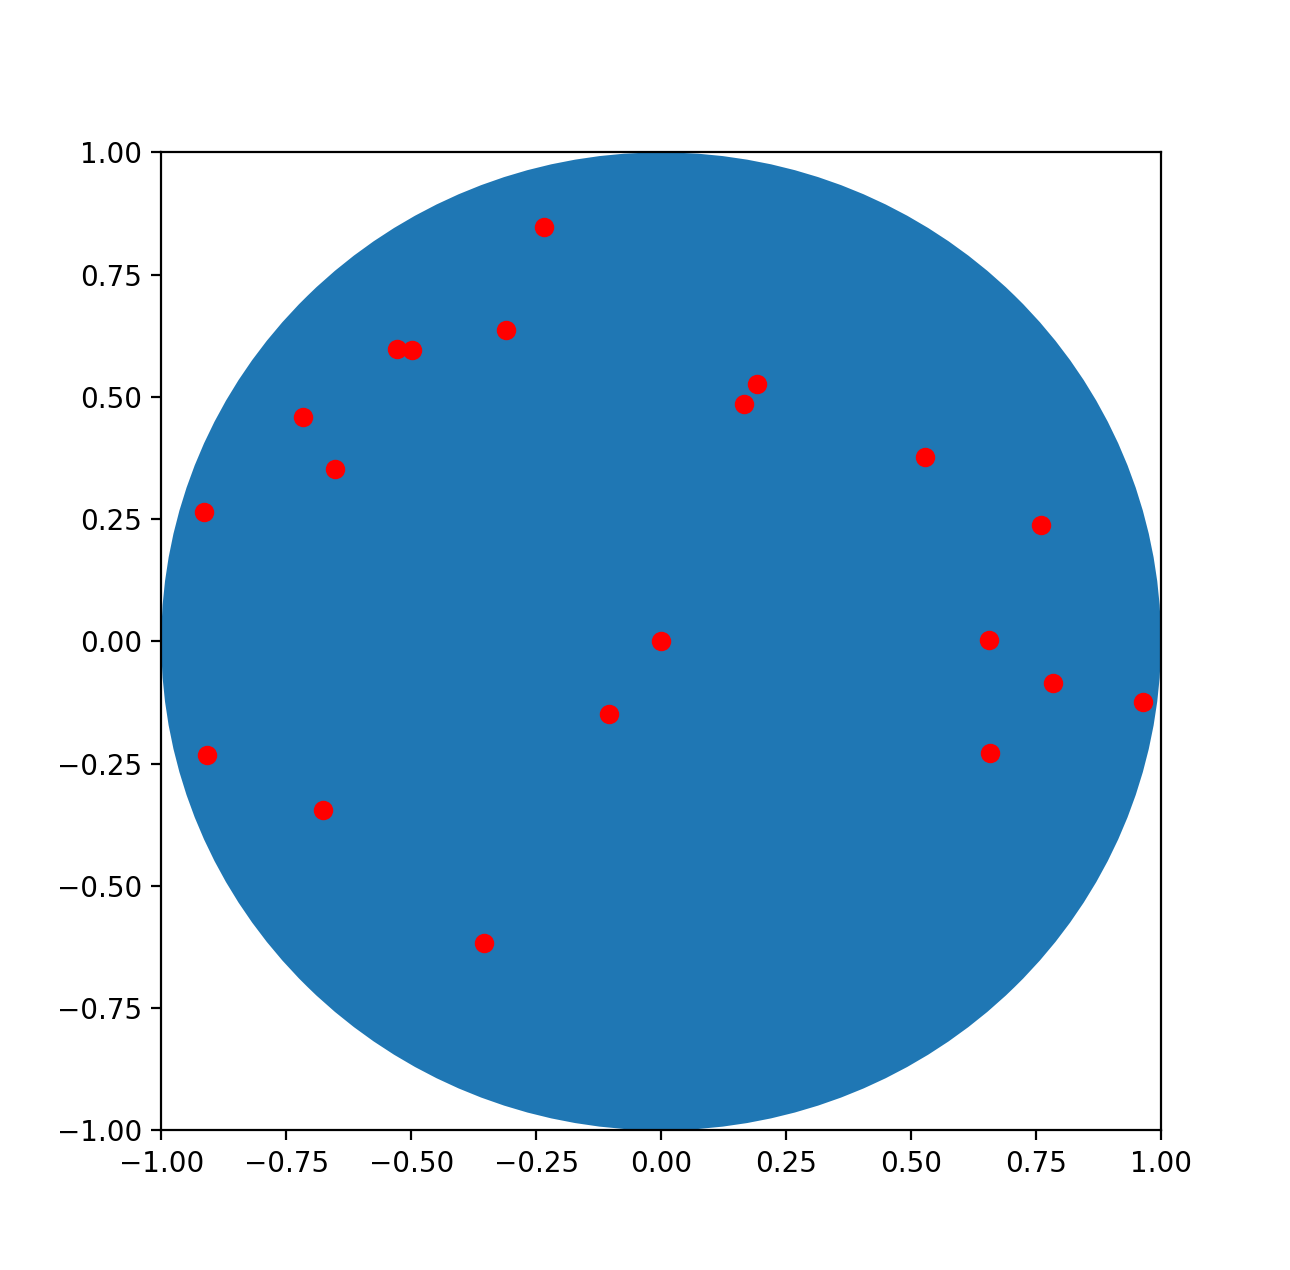
\includegraphics[scale = 0.4]{slikatockekrog}\\ 
\scriptsize{\textit{Slika 1: } Naključno izbrane točke znotraj kroga s pomerom $1$.}
\end{center}
\item Za zgenerirane točke izračunamo dolžine med vsakim parom točk in jih zapišemo v matriko. 
\item S Primovim algoritmom dobimo minimalno vpeto drevo:
\begin{center}
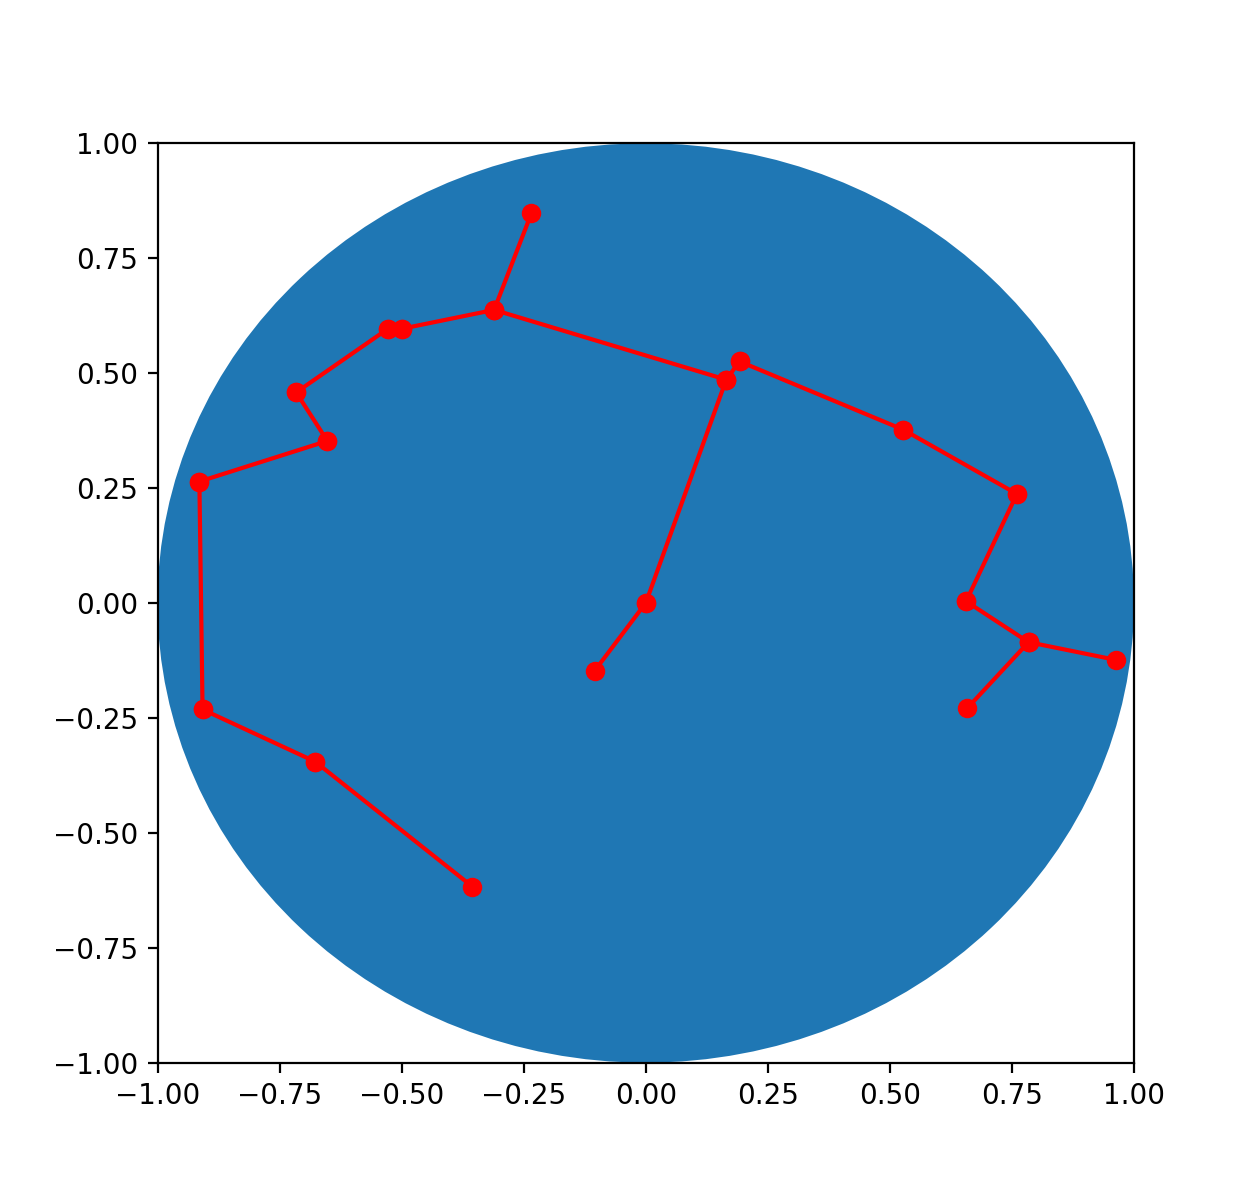
\includegraphics[scale = 0.4]{slikadrevokrog}\\ 
\scriptsize{\textit{Slika 2: } Minimalno vpeto drevo točk iz prejšnje slike.}
\end{center}
Izračunamo še vsoto kvadratov razdalj, tako da za vsako povezavo, ki je v minimalnem vpetem drevesu, pogledamo v matriko dolžin, da dobimo razdaljo in jo nato kvadriramo.
\end{enumerate} 
\textbf{Opomba: } Postopek računanja razdalje kvadratov vsot je enak za vse ostale like in je zato opisan samo enkrat. \\ \\
Spodnji graf (narisan v programu $R$) prikazuje odvisnost vsote kvadratov razdalj od zgeneriranega števila točk v krogu s polmerom $1$.
\begin{center}
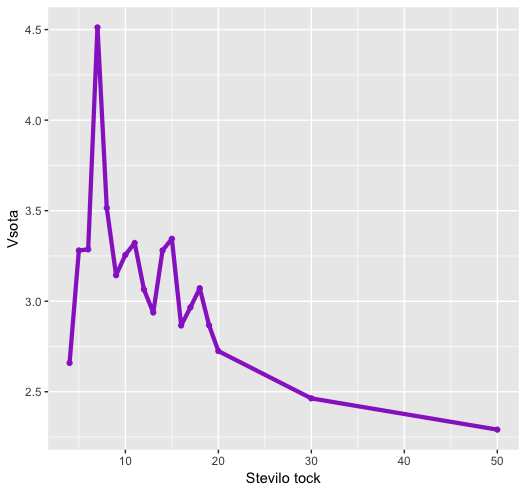
\includegraphics[scale = 0.4]{krog_st_tock}\\ 
\scriptsize{\textit{Graf 1: } Odvisnost vsote kvadratov razdalj od števila točk v krogu.}
\end{center}
Iz grafa lahko vidimo, da so vsote kvadratov razdalj z manjšim številom točk v krogu večje kot pri večjem številu točk. Ugotovili sva tudi, da bolj kot večava število točk, manjša je verjetnost za veliko vsoto. \\ \\


\subsubsection{Večanje polmerov}

Zanimalo naju je, kako se veča vsota kvadratov razdalj, če večeva polmer. Dokaj očitno je, da se bo vsota zelo hitro povečevala, kar je lepo razvidno tudi iz naslednjega grafa:
\begin{center}
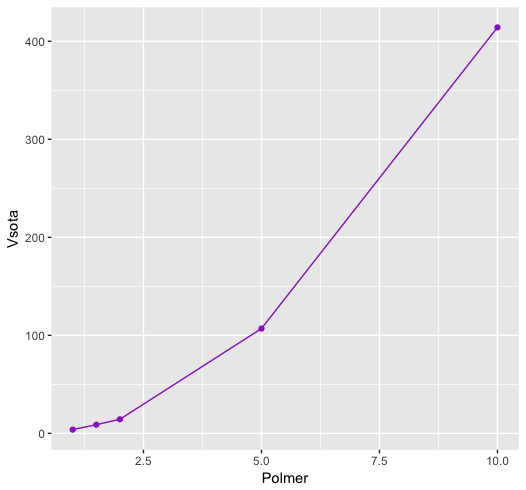
\includegraphics[scale = 0.3]{krog_polmer}\\ 
\scriptsize{\textit{Graf 2: } Odvisnost vsote kvadratov razdalj od polmera kroga.}
\end{center}

\subsubsection{Kdaj je vsota kvadratov razdalj enaka 6?}

S pomočjo primera, prikazanega v članku \textit{An Optimal Bound for the MST Algorithm to Compute Energy Efficient Broadcat Strees in Wireless Networks} sva našli točke, ki vrnejo največjo možno vsoto $6$. \\
Točk, ki vrnejo največjo vsoto v enotksem krogu je $7$: $(0,0), (1,0), (-1,0), (0.5, \frac{\sqrt{3}}{2}), (-0.5, \frac{\sqrt{3}}{2}), (0.5, -\frac{\sqrt{3}}{2}), (-0.5, -\frac{\sqrt{3}}{2})$. \\ \\
Najin algoritem za izračun vsote na minimalnem vpetem drevesu sva preizkusili na teh točkah (funkcija, ki izračuna to vsoto se nahaja v datoteki \colorbox{gray!10}{$skripta.py$}). Ugotovili sva, da je možnosti za minimalno vpeto drevo več, saj so dolžine med točkami, ki ležijo na krožnici med sosedami oddaljene enako kot od središča (torej med $(0,0)$ in $(1,0)$ je dolžina enaka kot med $(1,0)$ in $(0.5, \frac{\sqrt{3}}{2})$). Zaradi numeričnih napak v računanju dolžin, pa sva dobili nekatere razdalje $0.9999999$, kar je vodilo do izbire poti minimalnega vpetega drevesa, ki je prikazana na spodnjem grafu:
\begin{center}
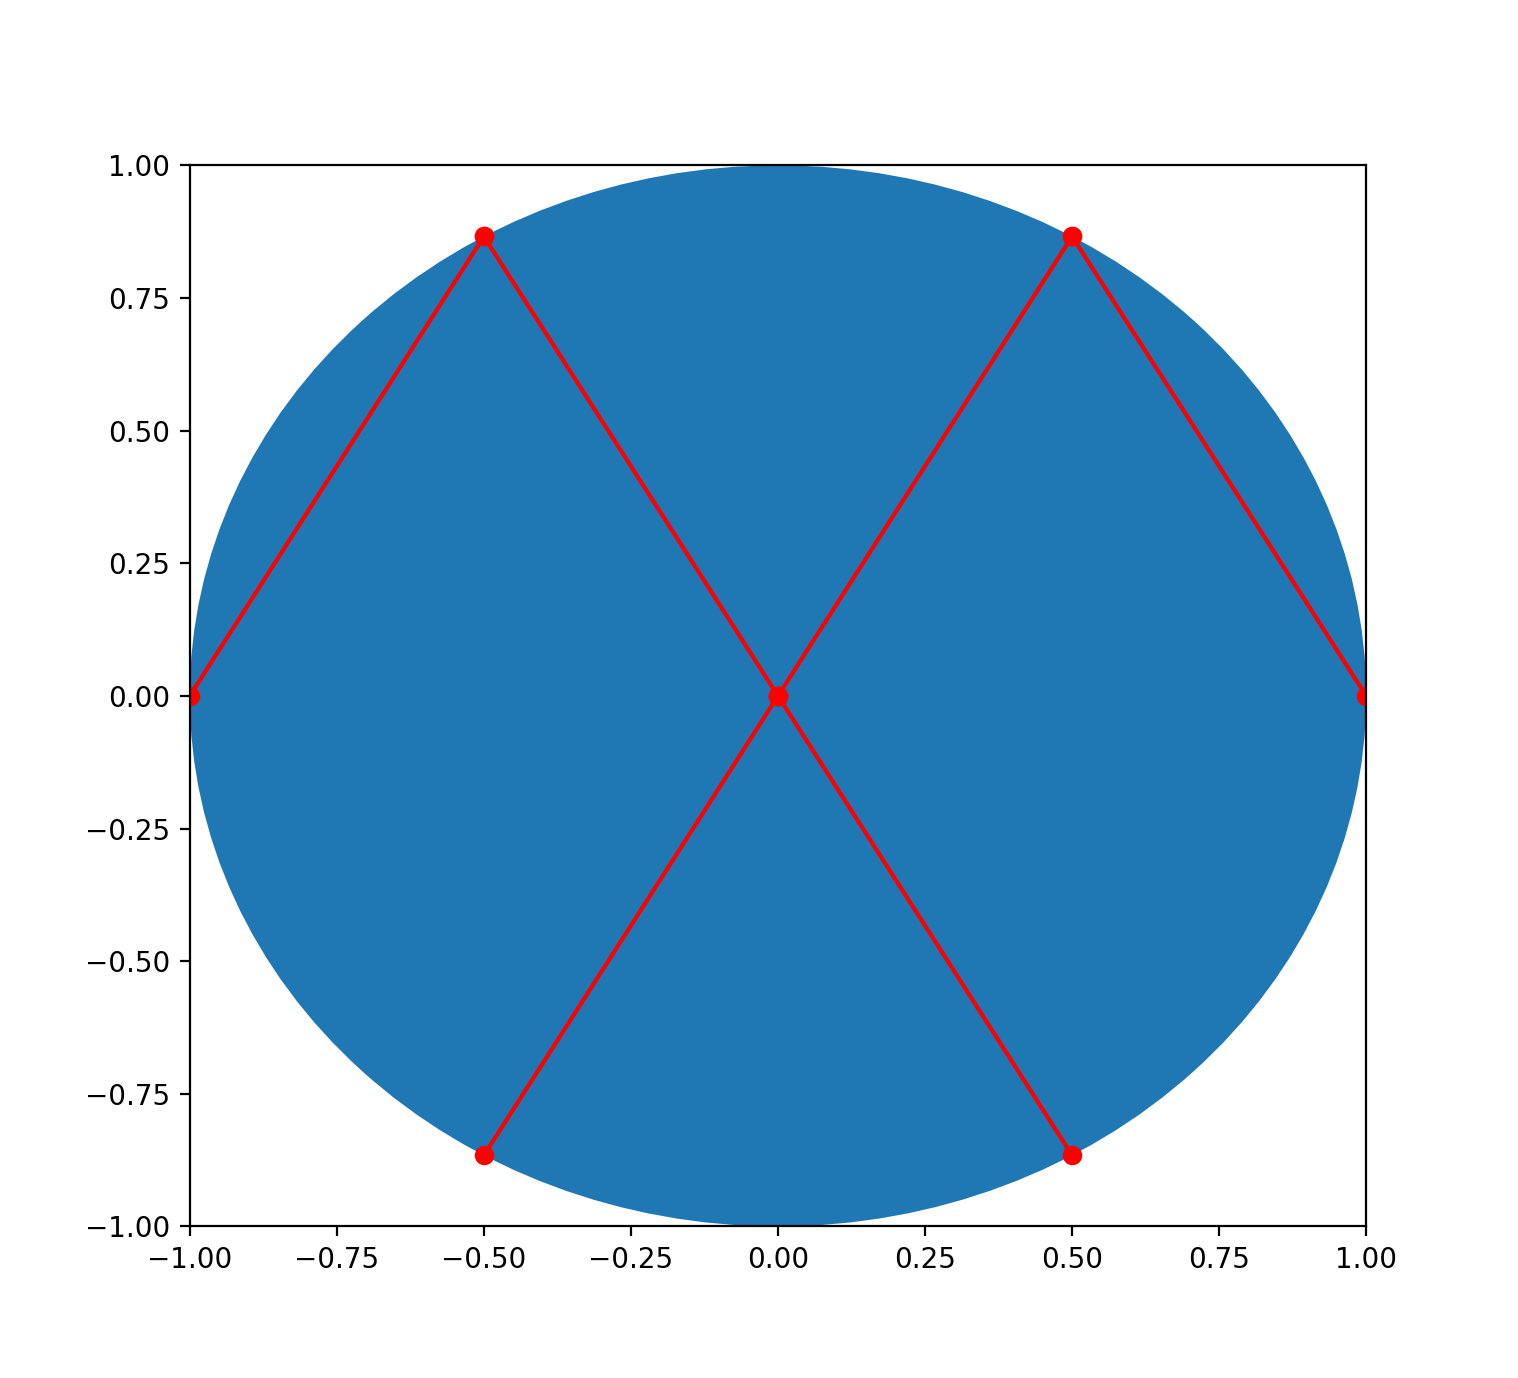
\includegraphics[scale = 0.3]{krog_vsota6}\\ 
\scriptsize{\textit{Slika 3: }  Odvisnost vsote kvadratov razdalj od števila točk v krogu.}
\end{center}


\subsection{Ostali liki}

Zanimali so naju tudi rezultati ostalih likov, predvsem primerjava različnih likov z enakimi ploščinami. Zato sva uporabili funkcijo $ploscina$ v datoteki \colorbox{gray!10}{$ploscine.py$}, ki nama je za dan polmer kroga izracunala podatke za ostale like.
Za kvadrat je s ploščino bila enolično določena stranica, prav tako za enakostranični trikotnik. Pri pravokotniku in elipsi pa sva morali določiti, kakšno bo razmerje med vodoravno in navpično dimenzijo. Za pravokotnik sva izbrali eno stranico, ki je bila enaka polmeru kroga, drugo stranico pa kot produkt polmera in $\pi$. Tako sta se in ena in druga stranica spreminjali glede na polmer.
Za elipso sva vzeli $a$ polos enako dvakratniku polmera, $b$ polos pa polovici polmera. 
Vsak lik je vseboval koordinatno izhodišče $(0,0)$ ter vsi, razen trikotnika, so bili na središče centrirani. Trikotnik pa je točko $(0,0)$ imel na osnovnici, osnovnica pa je ležala na abscisni osi. \\ \\
S $1000$ ponovitvami za različno število točk in za večanje polmera sva ugotovili več stvari:
\begin{enumerate} 
\item Pomembno je, kakšna je maksimalna dolžina med točko $(0,0)$ (ki smo jo imeli v vsakem liku je bila v večini primerov centrirana) in najbolj oddaljeno točko v liku. To je opazno pri elipsi, saj je njena razdalja od središča do skrajnega roba lika vedno bila največja in pokazalo se je, da je največja tudi njena vsota. (Glej $Graf 3$)
\item Zgornje meje vsot podobnih likov so zelo podobne. Na primer krog in kvadrat - na $Graf 3$ se razlika skoraj ne opazi. 
\item Z večanjem točk, ki jih zgeneriramo znotraj lika, se vsota kvadratov razdalj minimalnega vpetega drevesa med temi točkami manjša. (Glej $Graf 4$)
\item Z večanjem števila točk se vsote različnih likov vse manj razlikujejo in so pri $50$-ih točkah že zelo blizu. 
\end{enumerate}


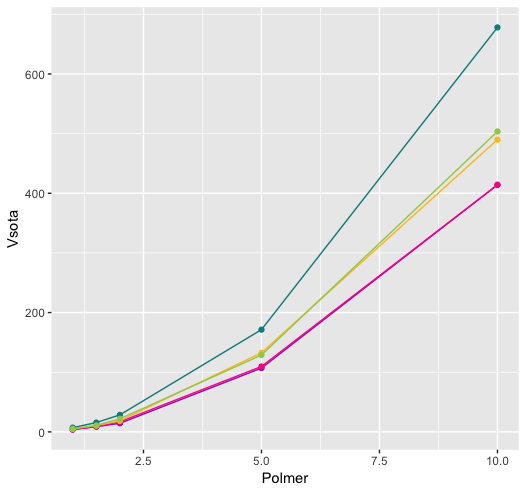
\includegraphics[width=0.4\textwidth]{odvisnost_od_polmera} \hspace{20mm}
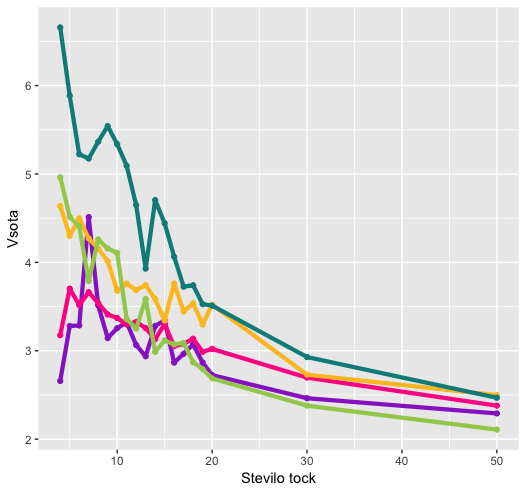
\includegraphics[width=0.4\textwidth]{odvisnost_od_tock} \\
\hspace{10mm} \scriptsize{\textit{Graf 3: }  Odvisnost vsote kvadratov razdalj od polmera.} \hspace{20mm}
\scriptsize{\textit{Graf 4: }  Odvisnost vsote kvadratov razdalj od števila točk.}


\subsection{Čas}

Za izvajanje različnih funkcij sva potrebovali različne količine časa (od glavnih treh funkcij je največ časa porabila funkcija za izračun vseh dolžin med točkami, kar je pričakovano, saj ima časovno zahtevnost $O(n^2)$. Zanimalo pa naju je, kako se veča porabljen čas za izračun vsega (generiranja točk, izračun dolžin med njimi in izračun vsote s pomočjo minimalnega vpetega drevesa) z večanjem števila danih točk. \\
V \colorbox{gray!10}{$skripta.py$} se nahaja funkcija $cas_glede_st_tock$, ki izracuna, koliko časa v povprečju porabi najin celoten algoritem. Za vsako število točk (število točk v posameznem poskusu $4, 5, 6, 7, 8, 9, 10, 11, 12, 13, 14, 15, 16, 17, 18, 19, 20, 50, 60, 70, 100, 150, 200, 250$) sva $100$-krat zagnali funkcijo in izračunali povprečno število časa. Pričakovali sva, da bo potreben čas zelo hitro naraščal, spodnji graf pa potrjuje najina pričakovanja.
\begin{center}
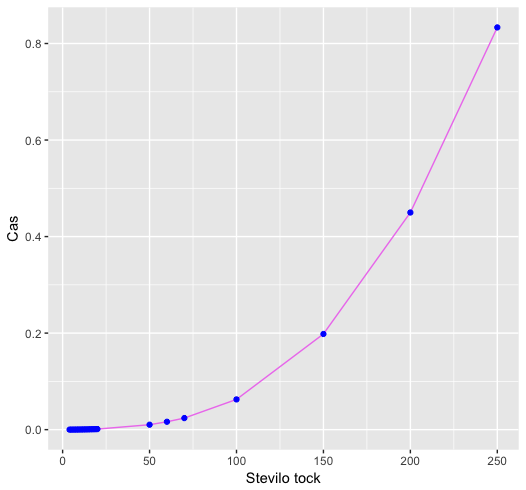
\includegraphics[width=0.4\textwidth]{graf_cas} \\
\scriptsize{\textit{Graf 5: }  Potreben čas algoritma pri določeni izbiri števila točk.}
\end{center}
\section{Ugotovitve in zaključek}

Zanimivo bi bilo tudi spreminjati fiksirano točko (ki je v našem primeru bila na sredini lika (razen v trikotniku)) in ugotavljati, kako se razlikujejo vsote kvadratov razdalj povezav minimalnega vpetega drevesa. 
Najine hipoteze so se izkazale v grobem za pravilne, čeprav je težje pokazati neko zgornjo mejo za elipso in pravokotnik, saj je vsota dolžin daljic odvisna od izbire stranic. V poročilu sva pokazali le eno izmed možnosti, lahko pa bi bila vsota še večja, če bi fiksirali stranico višine in povečevali le dolžino. Če bi želeli bolj natančno mejo tudi za ostale like, bi bilo potrebno najti posebne primere, kot je pri krogu, za vsoto 6. Tukaj bi prišli do problema pri številu točk, da pridemo do maksimalne zgornje meje, in potreben bi bil tudi dokaz, da je to res najvišja meja. 
\\




















\end{document}